\section{Topological Validation of Midsurface}

Topological validation can be performed using two methods:
\begin{itemize}
[noitemsep,topsep=2pt,parsep=2pt,partopsep=2pt]
\item \textbf{Solid-to-Surface}: Find the relationship between the topological entities of a thin-solid and its corresponding Midsurface. Check whether the \replaced[remark={Review B:  On page 8 ``Predicated'' should be ``Predicted''}]{predicted}{predicated} Midsurface entities validate the non-manifold equation (\ref{eqn_nonmanifold}).
\item  \textbf{Surface-to-Solid}: Predict the topological entities of a possible thin-walled solid that could be generated by thickening of the given Midsurface.  These predicted entities can be validated against the entities of the original thin-solid as well as with the manifold equation (\ref{eqn_manifold}).
\end{itemize}

%\subsection{Usefulness of Topological Validation}
Following are the ways in which some of the midsurface errors can be detected using the predicted entities:
\begin{itemize}
[noitemsep,topsep=2pt,parsep=2pt,partopsep=2pt]
\item \textbf{Missing Surfaces}: Missing surfaces result in lesser number of edges and vertices
\item \textbf{Missing Connections}: Gaps result in lesser radial edges and vertices 
\end{itemize}


% ************* OLD FAILED ATTEMPT ********************************
%In the Thin wall manifold solid faces are classified as as $f_p$ (Principal-Main faces) and $f_t$ (Thickness or capping faces). Edges are classified as $e_p$ (Principal-Main edges) and $e_t$ (along thickness or capping edges). Vertices are classified as $v_t$ (thickness vertex) when they are connected to at-least one $e_t$ and $v_p$ (principal or radial vertex), when they are connected to only $e_p$s.
%
%\subsubsection{Steps: Topological dimension reduction}
%\begin{itemize}
%[noitemsep,topsep=2pt,parsep=2pt,partopsep=2pt,leftmargin=*]
%\item Given a manifold solid, half of the $f_p$s are retained in the corresponding midsurface. Thickness faces $f_t$s and edges $e_t$s are gone. 
%%\item {\em Genuses} are the holes and the {\em rings} in the midsurface
%\item Half of the thickness vertices $v_t$s will remain in the midsurface. But the difficulty comes in predicting vertices at the junctions (corresponding to $v_p$s). Additional information about radial group of  $v_p$s is not directly available in the solid model (unless loop traversal detects cycles). 
%\item For example, in case of {\em \bf L} shape, half the $v_p$s are present in the midsurface as radial vertices, but in case of {\em \bf T} shape thats not true. So the procedure which is valid for  junctions up to degree two, is not so for the higher degree junctions. Examples below demonstrate this.
%\item Expand the Solid equation (\ref{eqn_manifold}) to include newly defined faces, edges: $ (v_p + v_t) - (e_p  + e_t) + (f_p  + f_t) = 2 (s - g) + r$
%\item For midsurface of this Solid, number of topological entities are changed as follows:
%	\begin{itemize}
%	[noitemsep,topsep=2pt,parsep=2pt,partopsep=2pt,label={}, leftmargin=*]
%	\item $v_{nm} = (v_p + v_t)/2$
% 	\item $e_{nm} = e_p/2$
%  	\item $e_t  = f_t  = r = 0$
%  	\item $f_{nm} = f_p/2$
%  	\end{itemize}
%\item Validate if the non-manifold equation $v_{nm} - e+{nm} + f_{nm} == (s_{nm} - g_{nm}) $ is honored.
%\end{itemize}
%
%\subsubsection{Examples}
%\begin{itemize}
%[noitemsep,topsep=2pt,parsep=2pt,partopsep=2pt,leftmargin=*]
%\item For Simple plate:
%	\begin{itemize}
%	[noitemsep,topsep=2pt,parsep=2pt,partopsep=2pt,label={}, leftmargin=*]
%%	\item \textcolor{blue}{``picture of the plate''}
%	\item $f_p =2,f_t=4,e_p=8,e_t=4,v_t=8,v_p=0,s=1,g=0$
% 	\item $v_{nm} = (v_t + v_p)/2 = 8 /2 = 4$
%  	\item $e_{nm} = e_p/2 = 8/2 = 4$
%  	\item $f_{nm} = f_p/2 = 2/2 = 1$
%  	\item $s_{nm} = 1, g_{nm} = 0$
%  	\item $v_{nm} - e_{nm} + f_{nm} = 4 - 4 +1 = 1 = (s_{nm} - g_{nm})$.
%  	\item \textbf{Result}: \textcolor{green}{Valid}
%  	\end{itemize}
%
%\item For 'L' shaped plate:
%	\begin{itemize}
%	[noitemsep,topsep=2pt,parsep=2pt,partopsep=2pt,label={}, leftmargin=*]
%%	\item \textcolor{blue}{``picture of L''}
%	\item $f_p =4,f_t=4,e_p=14,e_t=4,v_t=8,v_p=4,s=1,g=0$
% 	\item $v_{nm} = (v_t + v_p)/2 = (8+4) /2 = 6$
%  	\item $e_{nm} = e_p/2 = 14/2 = 7$
%  	\item $f_{nm} = f_p/2 = 4/2 = 2$
%  	\item $s_{nm} = 1, g_{nm} = 0$
%  	\item $v_{nm} - e_{nm} + f_{nm} = 6 - 7 + 2= 1 = (s_{nm} - g_{nm})$.
%  	\item \textbf{Result}: \textcolor{green}{Valid}
%  	\end{itemize}
%  	
%  	\item For 'T' shaped plate: 
%	\begin{itemize}
%	[noitemsep,topsep=2pt,parsep=2pt,partopsep=2pt,label={}, leftmargin=*]
%%	\item \textcolor{blue}{``picture of T''}
%	\item $f_p =5,f_t=5,e_p=20,e_t=6,v_t=12,v_p=4,s=1,g=0$
% 	\item $v_{nm} = (v_t + v_p)/2 = (12+4) /2 = 8$
%  	\item $e_{nm} = e_p/2 = 20/2 = 10$
%  	\item \textcolor{red}{$f_{nm} = f_p/2 = 5/2 = 2.5$}
%  	\item $s_{nm} = 1, g_{nm} = 0$
%  	\item $v_{nm} - e_{nm} + f_{nm} = 6 - 7 + 2= 1 = (s_{nm} - g_{nm})$.
%  	\item \textbf{Result}: \textcolor{red}{Invalid}
%  	\end{itemize}
%
%\end{itemize}
%
%\textbf{Conclusion}: Manifold equation of Thin Solid cannot be simplistically converted to non-manifold equation of its midsurface. Thus this direction of validation has limitations. Following section examines if the other direction of validation is possible or not.


\subsection{Sheet Metal Solid to Midsurface Transformation}
Given a thin-walled sheet metal solid, below is an approach to propose the dimension-reduction-transformation equations for predicting the topological entities of its corresponding midsurface. The given original solid is first decomposed into sub-volumes, called as ``Cells''  \added[remark={Review C: Minor revision: In section 2.1.2 Examples, adding figures of decomposed cells from solids would be helpful for readers to understand the method clearly. Especially, configuration of sCells of Y- and rounded L-shape solid is hard to understand 
in a text form. }]{(Tabel~\ref{tbl_celldecompexample})} and then the dimension-reduction-transformation is derived.% Topology generated by the volumetric decomposition is called {\em Cellular Topology}. 


Many commercial as well as academic methods are available for cellular-volumetric decomposition \cite{Woo2002, Chong2004, Cao2011,  Boussuge2013, Kim2014}. \added[remark={ Review B: In section 2.1 please expand the explanation of the cellular-volumetric decomposition method used and the result obtained for 
the case study part. In the context of sheet metal parts is it 
possible to obtain a cell with dimensionality 0 or 1? }]{
Woo (maximal cells \cite{Woo2003}), Boussuge (Extrusion decomposition \cite{Boussuge2013a}), Wu (Sweep Decomposition \cite{Wu2014}), Woo (Protrusion decomposition \cite{Woo2014}), etc. are some of the known cellular decomposition methods used for feature recognition (FR).} 

\added[remark={ Review B: The paper could be improved by providing a more detailed explanation of the cellular decomposition method and highlighting its limitations (for example cellular decomposition can be computationally expensive 
and may not produce a ``clean'' result). How does this impact the 
application of the presented method? }]{Cellular decomposition starts facing problems as the complexity of the original solid increases. The method becomes very slow as the number of cells increases \cite{Woo2003}. If the cutting faces are extended infinitely and intersected with the whole solid then they generate a large number of unnecessary cells. If the splits are not clean, it may generate degenerate entities such as edges and vertices. The topological validation method presented here assumes `clean' cellular decomposition and if it is not so, then the validation results could be unpredictable.}


%\begin{center}\includegraphics[width=0.6\linewidth]{../Common/images/VolDecomp.pdf}\end{center}
%\vspace{-0.8cm}
%\begin{center}\includegraphics[width=0.6\linewidth]{../Common/images/VolDecomp1.pdf}\end{center}
%\vspace{-1.2cm}

\subsubsection{Steps: Topological Dimension Reduction}
Topological transformation of solid (3D cells) to its corresponding midsurface (2D cells) is as follows:

\begin{itemize}
[noitemsep,topsep=2pt,parsep=2pt,partopsep=2pt]

	\item  $sCell_{3,n}$:	Solid cell with $n$ touching sides transforms into midsurface cell   $mCell_{2,n}$, a surface having $n$ empty edges. Its topological entities are denoted as:
\begin{equation}
f=1;
e=4-n;
v=4-2n
\label{eqn_cellularna}
\end{equation} 

	\item   $sCell_{3,h}$ : Negative solid  cell representing a through hole transforms into midsurface cell  $mCell_{2,h}$, a hole in the surface. Its topological entities are denoted as:
\begin{equation}
e=1; v=1
\label{eqn_cellularah}
\end{equation} 

	\item $iCell_{3,n}$ :	Interface solid cell with $n$ adjacent touching sides transforms into midsurface cell  $mCell_{1,n}$, a radial edge with $n$ leaves. Its topological entities are denoted as:

\begin{equation}
e=1;
v=2
\label{eqn_cellulara}
\end{equation}

	\item  $iCell_{2,2}$ :	Interface face cell touched from both sides  transforms into midsurface cell  $mCell_{1,2}$, a radial edge with 2 leaves. Its topological entities are denoted as:
\begin{equation}
e=1;
v=2
\label{eqn_cellularaf}
\end{equation}


\end{itemize}

%(Eqn   \ref{eqn_cellulara}, \ref{eqn_cellularaf}, \ref{eqn_cellularna}, \ref{eqn_cellularah} )

\subsubsection{Examples}
Table \ref{table_simpleshapes1} lists various basic shapes and their dimension-reduction-transformations into the corresponding midsurface
It is evident that the predicted midsurface entities of these simple shapes match with the actual ones, thus the derived formulation works for these simple shapes. 

\begin{minipage}{0.92\linewidth}
\begin{center}

\begin{tabular}[h]{@{}p{0.1\linewidth} p{0.1\linewidth} | p{0.15\linewidth} |  p{0.15\linewidth} | p{0.35\linewidth}@{}} \toprule
{\bf Solid} & {\bf mSurf}  & {\bf sCells} & {\bf mCells}  & {\bf Predicted mSurf Entities} \\ \midrule  

\adjustbox{valign=c}{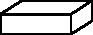
\includegraphics[width=\linewidth]{../Common/images/SimplePlate1.pdf}}  &  
\adjustbox{valign=c}{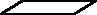
\includegraphics[width=\linewidth]{../Common/images/SimplePlane1.pdf}} &  
$sCell_{3,0}$ & $ mCell_{2,0}$ & 
$ 1f+(4-0)e+(4- 2\times 0)v \newline = 1f+4e+4v$
\\ %\midrule

\adjustbox{valign=c}{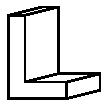
\includegraphics[width=\linewidth]{../Common/images/LPlate1.pdf}}  &  
\adjustbox{valign=c}{
\includegraphics[width=\linewidth]{../Common/images/LPlane1.pdf}} &  

$2 \times sCell_{3,1} \newline + iCell_{3,2}$ & $2 \times mCell_{2,1} \newline + mCell_{1,2}$  & 
$ 2 \times (1f + (4-1)e+(4-2\times 1)v ) \newline + (1e + 2v) \newline = 2f+7e+6v$ 
\\ %\midrule


\adjustbox{valign=c}{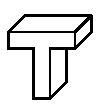
\includegraphics[width=\linewidth]{../Common/images/TPlate1.pdf}}  &  
\adjustbox{valign=c}{
\includegraphics[width=\linewidth]{../Common/images/TPlane1.pdf}} &  

$3 \times sCell_{3,1} + iCell_{3,3}$   &  $3 \times mCell_{2,1}  + mCell_{1,3}$  & 
$3 \times (1f+(4-1)e+ (4-2\times 1)v)  + (1e+2v)  = 3f+10e+8v$ 
\\ %\midrule

\adjustbox{valign=c}{
\includegraphics[width=\linewidth]{../Common/images/YwithHole1.pdf}}  &  
\adjustbox{valign=c}{
\includegraphics[width=\linewidth]{../Common/images/YwithHolem1.pdf}} &  

$3 \times sCell_{3,1}  + iCell_{3,3}  + sCell_{3,h}$   &  
$3 \times mCell_{2,1}  + mCell_{1,3}  + mCell_{2,h}$  & 
$3 \times (1f+(4-1)e+ (4-2\times 1)v)  + (1e+2v)  + (1e+1v)  = 3f+11e+9v$
\\ %\midrule

\adjustbox{valign=c}{
\includegraphics[width=\linewidth]{../Common/images/LwithRound1.pdf}}  &  
\adjustbox{valign=c}{
\includegraphics[width=\linewidth]{../Common/images/LwithRoundm1.pdf}} &  

$2 \times sCell_{3,1}  + 2 \times  iCell_{2,2}  + sCell_{3,2}$   &  
$2 \times mCell_{2,1}  + 2 \times mCell_{1,2}  + mCell_{2,2}$  & 
$2 \times (1f+(4-1)e+ (4-2\times 1)v)  + 2 \times (1e+2v)  + (1f+(4-2)e+ (4-2\times 2)v)  = 3f+10e+8v$
\\ 

\bottomrule
\end{tabular}
\captionof{table}{Dimension-reduction-transformations.}
\label{table_simpleshapes1}
\end{center}

\end{minipage}

 Following is the verification for a relatively-complex practical shape. 

\begin{tabular}[htp]{@{}p{0.48\linewidth}  p{0.48\linewidth}@{}} \toprule
{\centering  \bf Solid} & { \centering  \bf Cellular Classification} \\ \midrule
\includegraphics[width=\linewidth]{../Common/images/SimpleBracketshaded.pdf} &
\includegraphics[width=\linewidth]{../Common/images/SimpleBracket.pdf}\\ \bottomrule
\end{tabular}

\begin{itemize}
[noitemsep,topsep=2pt,parsep=2pt,partopsep=2pt,leftmargin=*]
	\item \textbf {Solid cells}: \newline  $5 \times sCell_{3,h} + 3 \times sCell_{3,1} + 13 \times sCell_{3,2} + 14 \times iCell_{2,2} $
	\item \textbf {Transformed Midsurface Cells}: \newline $5 \times mCell_{2,h} + 3 \times mCell_{2,1} + 13 \times mCell_{2,2} + 14 \times mCell_{1,2}$
	\item \textbf {Predicted midsurface Entities are}:  \newline $5(1e+1v) + 3 (1f+3e+2v) + 13 (1f+2e+0v) + 14(1e+2v) = 
16f + 54e + 39v$
\end{itemize}


The derived formulation (Eqn   \ref{eqn_cellulara}, \ref{eqn_cellularaf}, \ref{eqn_cellularna}, \ref{eqn_cellularah} ) predicts correct topological entities for the midsurface. These, when substituted in the non-manifold equation (Eqn \ref{eqn_nonmanifold}) also prove to be valid. With $s=1, r=5, h=5$, the equation matches both sides:
$ 39 - 54 + (16 -5) = 1 (1-5)$


\subsection{Midsurface to Sheet Metal Solid Transformation}
In this approach, given a midsurface, topological entities  of its corresponding sheet metal solid are predicted. These predicted entities are verified to check if they validate manifold equation (Eqn \ref{eqn_manifold}). Topological entities of midsurface contains far richer (classifiable) topological information than its corresponding solid model. For example, midsurface of ``T'' shaped solid, which can be represented as Figure \ref{fig_nonmanifold} has following classified entities:



\begin{itemize} 
[noitemsep,topsep=2pt,parsep=2pt,partopsep=2pt,label=\textbullet]\label{list_topos}
\item Faces ($f$): Bound by two face-uses $f_u$.

\item Sharp Vertex ($v_s$): Connected to two edges of the same face
\item Sharp Edge ($e_s$): Connected to two sharp vertices

\item Radial Vertex ($v_{r}$): Connected edges of different faces
\item Degree ($n_{r}$) at the radial edge is the number of faces attached to it 
\item Cross Radial Edge ($e_{r}$): Connected between two radial vertices and connects two different faces
\item Side-Radial  Edge ($e_{rr}$): Connected between two radial vertices and is of same face
\item Sharp-Radial Edge ($e_{sr}$): Between sharp and radial vertex
\item Internal Edge ($e_i$): Part of the inner loop
\item Internal Vertex ($v_i$):Connected to the internal edge
\item Internal Loop ($r_i$) : Characterized by internal edges and vertices
\end{itemize}

\begin{minipage}[t]{\linewidth}
\centering 
\includegraphics[width=\linewidth]{../Common/images/NonManifoldT1.pdf}
\vspace{2mm}
\captionof{figure}{Non-Manifold topological entities}
\label{fig_nonmanifold}
\end{minipage}


\subsubsection{Steps: Topological Dimension Addition}
Sheet Metal solid can be imagined to be thickened midsurface \cite{SHLee2001}. The topological entities of the generated solid are calculated as per following steps: %via relations in the Table \ref{table_TopoVal}.

\begin{itemize}
[noitemsep,topsep=2pt,parsep=2pt,partopsep=2pt,leftmargin=*]
\item Face-uses become principal faces. 
 
\item Sharp vertices create capping edges.

\item Apart from edge-use loop corresponding to face-use, a new loop is proposed for side-capping faces. The loop is formed between two sharp vertices ($v_s$) using  more than one sharp  ($e_{sr}$) or side radial ($e_{rr}$) edges but not using the cross radial edge ($e_r$). Such independent paths creating individual side faces are called $l_p$.
\item Loop between two sharp vertices. This gives rise to a singular capping face  (Fig.~\ref{fig:loopstofaces} a).
\item Loop between three branched sharp vertices. This gives rise to a combined capping face (Fig.~\ref{fig:loopstofaces}  b).
\item Loop between two sharp vertices with multiple radial vertices in between them. This gives rise to a combined capping face (Fig.~\ref{fig:loopstofaces}  c).
\end{itemize}
	

\begin{minipage}[t]{\linewidth}
\centering 
\includegraphics[width=0.45\linewidth]{../Common/images/NonManifoldLoopsToFaces1.pdf}

\captionof{figure}{Loops to Faces}
\label{fig:loopstofaces}
\end{minipage}



Topological entities in the thickened solid are predicted as follows:% (Summary in Table \ref{table_TopoVal}):
\begin{itemize}
[noitemsep,topsep=2pt,parsep=2pt,partopsep=2pt,label=\textbullet]
\item Manifold-Vertices  ($v_m$) = Double the sharp and internal vertices (one up  and  one below) + vertices for junctions of which are denoted by the summation of  number of radial vertices times their corresponding degrees
\begin{equation}
v_m = 2 (v_s + v_i) + \sum n_{r} v_{r} \label{eqn_vm}
\end{equation}
\item \textbf{Manifold-Edges ($e_m$)}= two times sharp, sharp-radial and internal edges (offset up and down) + degree times radial edges for offsets at junctions + sharp vertices for vertical-capping edges + internal vertices for vertical seam edges
\begin{equation}
e_m = 2 (e_s + e_{sr} + + e_{rr} + e_i) + \sum n_r e_r  + v_s + v_i\label{eqn_em}
\end{equation}
\item \textbf{Manifold-Faces ($f_m$)} = Double the faces (offset up and down) + sharp edges for capping faces + paths to have one combined face + internal edges for capping internal faces
\begin{equation}
f_m = 2f + e_s + l_p + e_i \label{eqn_fm}
\end{equation}
\item \textbf{Manifold-Shells ($s_m$)} = Remains the same
\item \textbf{Manifold-Rings ($r_m$)} = Two times the internal rings
\begin{equation}
r_m = 2r_i\label{eqn_rm}
\end{equation}
\item \textbf{Manifold-Genus ($h_m$)} = Internal ring as it becomes a hole
\begin{equation}
h_m = r_i\label{eqn_hm}
\end{equation}

\end{itemize}
\subsubsection{Procedure to Validate Midsurface}
\begin{enumerate}
\item Count topological entities of the midsurface as per the classification suggested : \\$f, e_s , e_{sr} , e_{rr}, e_r , e_i, v_s , v_r , v_i, s , h , r$ (more details in Section \ref{list_topos}) .
\item Predict topological entities of the corresponding thin-walled solid using equations ( \ref{eqn_vm}, \ref{eqn_em}, \ref{eqn_fm}, \ref{eqn_rm}, \ref{eqn_hm}).
	\begin{enumerate}
%		\item Predicted solid-faces: $f_m \\= 2f+e_s+e_{sr}/n_{r} +e_i $
		\item Predicted solid-faces: $f_m \newline = 2f+e_s+ l_p +e_i $
		\item Predicted solid-edges: $e_m \newline = 2(e_s+e_{sr}+e_{rr}+e_i )+ \sum n_{r} e_{r}+v_s+v_i $
		\item Predicted solid-vertices: $v_m \newline= 2v_s+ \sum n_{r} v_r+2v_i$
		\item Predicted solid-shells-holes: \newline$s_m =s = 1, h_m = r_i  = 0, r_m = 2r_i = 0$
		\item Non-manifold equation of the left side  $\chi_{nml} \newline= v-e+f $
		\item Non-manifold equation of the  right side  $\chi_{nmr} \newline=s-h+r$
		\item Manifold equation of the  left side  $\chi_{ml} \newline= v_m-e_m+f_m $
		\item Manifold equation of the  right side  $\chi_{mr}\newline=2(s_m-h_m )+r_m$
%		\item Sheet metal midsurface characteristic $\chi_{smm} \\=
%		e_s+e_i+(2-n_{r} ) e_{r}+e_{sr}/n_{r} =v_s+(2-n_{r} ) v_{r}+v_i$
	\end{enumerate}
\item Verify that the topological entities of the midsurface satisfy the non-manifold equation (Equation \ref{eqn_nonmanifold}), by deducing that the left ($\chi_{nml}$) and right  ($\chi_{nmr}$) hand side of the equation matches.
\item Verify that the predicted topological entities of the  thin-walled solid satisfy the manifold equation (Equation \ref{eqn_manifold}), by deducing that the left ($\chi_{ml}$) and right  ($\chi_{mr}$) hand side of the equation match; thus proving that the transformation equations are valid. 
%Same validity can be shown using just the $\chi_{smm}$ characteristic, as below.
%\item Verify that  $\chi_{smm}$ characteristic equation (Equation \ref{eqn_nonmanifolddiff}) matches. 
\end{enumerate}



\subsubsection{Examples}
Table \ref{table_simpleshapes2} displays the validation of midsurface using proposed dimension-addition-transformation equations. It is evident that the derived formulation works for simple shapes. 

\begin{minipage}{0.65\linewidth}
\begin{center}

\begin{tabular}[t]{@{} p{0.08\linewidth}  
p{0.02\linewidth}  p{0.02\linewidth}  p{0.02\linewidth}   p{0.02\linewidth}  p{0.02\linewidth}  p{0.02\linewidth}     p{0.02\linewidth}  p{0.02\linewidth}  p{0.02\linewidth} p{0.02\linewidth}  p{0.02\linewidth}  p{0.02\linewidth}  p{0.02\linewidth}   p{0.02\linewidth} @{}} \toprule
{\bf m} & 
{\bf $f$}  		& {\bf $l_p$ } 	& {\bf $e_s$ }  	& {\bf $e_{sr}$} & {\bf $e_r$}  & 
{\bf $e_{rr}$} 	& {\bf $e_i$ } 	& {\bf $v_s$ } 	& {\bf $v_r$}  	&  {\bf $v_i$}  & 
{\bf $f_{m}$} 	& {\bf $e_m$ } 	& {\bf $v_m$ } 	& {\bf $\chi_{m*}$ } \\ \midrule 

\adjustbox{valign=c}{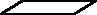
\includegraphics[width=\linewidth]{../Common/images/SimplePlane1.pdf}}  &  
1 & 0 & 4 & 0 & 0 & 0 & 0  & 4 & 0 & 0 & 6 & 12 & 8 & 2 \\ 

\adjustbox{valign=t}{
\includegraphics[width=\linewidth]{../Common/images/LPlane1.pdf}}  &  
2 & 2 & 2 & 4 & 1 & 0 & 0  & 4 & 2 & 0 & 8 & 18 & 12 & 2 \\ 


\adjustbox{valign=t}{
\includegraphics[width=\linewidth]{../Common/images/TPlane1.pdf}}  &  
3 & 2 & 3 & 6 & 1 & 0 & 0  & 6 & 2 & 0 & 11 & 27 & 18 & 2 \\ 

\adjustbox{valign=c}{
\includegraphics[width=\linewidth]{../Common/images/YwithHolem1.pdf}}  &  
3 & 2 & 3 & 6 & 1 & 0 & 1  & 6 & 2 & 1 & 12  &  30  & 20  & 2 \\ 

\adjustbox{valign=c}{
\includegraphics[width=\linewidth]{../Common/images/LwithRoundm1.pdf}}  &  
3 & 2 & 2 & 4 & 2 & 2 & 0  & 4 & 4 & 0 & 10  & 24  & 16  & 2 \\  
\bottomrule
\end{tabular}

\captionof{table}{validation of midsurface}
\label{table_simpleshapes2}
\end{center}
\end{minipage}

\vspace{1mm}

Following is the verification for a relatively-complex practical shape.

\begin{tabular}[htp]{@{}p{0.48\linewidth}  p{0.48\linewidth}@{}} \toprule
{\bf Midsurface} & {\bf Edge Classification} \\ \midrule
\includegraphics[width=\linewidth]{../Common/images/SimpleBracketMidsurfshaded.pdf} &
\includegraphics[width=\linewidth]{../Common/images/SimpleBracketMidsurf.pdf}\\ \bottomrule
\end{tabular}

\begin{enumerate}
[noitemsep,topsep=2pt,parsep=2pt,partopsep=2pt,label=\textbullet]
\item \textbf{Midsurface entities}: \\$f = 15, e_s = 3, e_{sr} = 10, e_r = 14, e_{rr} = 19, l_p = 9 ,e_i=5,v_s = 8,v_r =24, v_i= 5, s=1,h=5,r=5$
\item \textbf{Predicted solid-faces}: \\$f_m = 2f+e_s+ l_p +e_i $\\$= 2 \times 15 + 3 + 9 + 5 = 47$
\item \textbf{Predicted solid-edges}: \\ $e_m = 2(e_s+e_{sr}+e_{rr}+e_i )+ \sum n_{r} e_{r}+v_s+v_i $\\$= 2(3+10+19 + 5)+ (2\times 12 + 4 \times 2)+8+5 = 119$
\item \textbf{Predicted solid-vertices}: \\$v_m = 2(v_s+ v_i) + \sum n_{r} v_r$\\$=2\times (8 + 5)  + 2 \times 24=74$
\item \textbf{Predicted solid-shells-holes}: \\$s_m =s = 1, h_m = r_i  = 5, r_m = 2r_i = 10$
\item \textbf{Non-manifold equation of the left side}:  $\chi_{nml} $\\$= v-e+f $\\$= 32-46+15 = 1$
\item \textbf{Non-manifold equation of the  right side}:  $\chi_{nmr}$\\$=s-h+r$\\$=1-5+5 = 1$
\item \textbf{Manifold equation of the  left side}:  $\chi_{ml} $\\$= v_m-e_m+f_m $\\$=74-119+47= 2$
\item \textbf{Manifold equation of the  right side}:  $\chi_{mr}$\\$=2(s_m-h_m )+r_m$\\$= 2(1-5)+10 = 2$
%\item Sheet metal midsurface characteristic $\chi_{smm}$\\$=
%e_s+e_i+(2-n_{r} ) e_{r}+e_{sr}/n_{r} $\\$=v_s+(2-n_{r} ) v_{r}+v_i$\\$ 4+0+0+0=4+0+0= 4$
%\item \textbf{Result}: \textcolor{green}{Matches}
\end{enumerate}
It can be observed that the predicted solid entities validate the manifold equation ($\chi_{ml} = \chi_{mr} = 2$). Validation can also be performed by comparing the  topological entities of the thin-walled solid with the predicted ones.
